\documentclass[11pt]{article}
\usepackage[margin=1in]{geometry}
\usepackage{amsmath, amssymb, amsthm}
\usepackage{algorithm, algpseudocode}
\usepackage{graphicx}
\usepackage{xcolor}
\usepackage{listings}
\usepackage{hyperref}
\usepackage{booktabs}
\usepackage{float}

\definecolor{codegreen}{rgb}{0.2,0.6,0.2}
\definecolor{codered}{rgb}{0.7,0.15,0.15}
\definecolor{codegray}{rgb}{0.4,0.4,0.4}
\definecolor{codebg}{rgb}{0.97,0.97,0.97}

\lstset{
  language=R,
  basicstyle=\ttfamily\small,
  keywordstyle=\color{codered}\bfseries,
  commentstyle=\color{codegray}\itshape,
  stringstyle=\color{codegreen},
  backgroundcolor=\color{codebg},
  frame=single,
  rulecolor=\color{codegray!40},
  numbers=left,
  numberstyle=\tiny\color{codegray},
  breaklines=true,
  columns=fullflexible,
  showstringspaces=false,
  tabsize=2,
  xleftmargin=1.5em,
  framexleftmargin=1em,
}

\newcommand{\R}{\textsf{R}}

\title{Rejection Sampling: Theory and Implementation}
\author{Adam Kurth \\ PHP 2530 --- Bayesian Statistics}
\date{Spring 2026}

\begin{document}
\maketitle

% ----------------------------------------------------------------
\section{Motivation}

Many Bayesian posteriors and other distributions of interest lack closed-form samplers.  Rejection sampling provides a way to draw exact, independent samples from a target density~$f$ by using a simpler proposal density~$g$ that we \emph{can} sample from.  The only requirements are:
\begin{enumerate}
  \item We can evaluate $f(x)$ pointwise (up to a normalizing constant).
  \item There exists a proposal $g$ and a finite constant $c \ge 1$ such that $c\,g(x) \ge f(x)$ for all~$x$.
\end{enumerate}

% ----------------------------------------------------------------
\section{The Algorithm}

\begin{algorithm}[H]
\caption{Rejection Sampling}
\label{alg:reject}
\begin{algorithmic}[1]
\Repeat
  \State Draw $Y \sim g$ \Comment{proposal}
  \State Draw $U \sim \mathrm{Uniform}(0,1)$ \Comment{independent}
  \If{$U \le \dfrac{f(Y)}{c\,g(Y)}$} \Comment{accept with this probability}
    \State \textbf{accept} $X = Y$
  \Else
    \State \textbf{reject} $Y$ and repeat
  \EndIf
\Until{a sample is accepted}
\end{algorithmic}
\end{algorithm}

\subsection{Why It Works}

The key identity is
\[
  P(\text{accept} \mid Y = y) \;=\; \frac{f(y)}{c\,g(y)},
\]
so the marginal probability of acceptance at any step is
\[
  P(\text{accept})
  = \int \frac{f(y)}{c\,g(y)}\,g(y)\,dy
  = \frac{1}{c}\int f(y)\,dy
  = \frac{1}{c}.
\]
By Bayes' theorem, the density of an accepted value $X$ is
\[
  f_{X}(x)
  = \frac{P(\text{accept}\mid Y=x)\,g(x)}{P(\text{accept})}
  = \frac{\tfrac{f(x)}{c\,g(x)}\,g(x)}{1/c}
  = f(x).
\]
Thus accepted draws are distributed exactly as~$f$.  The expected number of proposals per accepted sample is~$c$, so the \textbf{acceptance rate} is~$1/c$.  Minimizing~$c$ is therefore critical for efficiency.

% ----------------------------------------------------------------
\section{Implementation in \R}

The companion script \texttt{rejection-sampling.r} demonstrates two examples with four figures.  We walk through each block below.

\subsection{Example 1: $\mathrm{Beta}(2.7,\, 6.3)$ via $\mathrm{Uniform}(0,1)$}

\paragraph{Setup.}
The target is $f(x) = \mathrm{Beta}(x;\,2.7,\,6.3)$ on $[0,1]$.  The proposal is $g(x) = 1$ (the Uniform density).  Since $g(x)=1$, the envelope constant is simply the maximum of~$f$:
\[
  c = \max_{x} f(x) = f\!\left(\frac{a-1}{a+b-2}\right),
\]
evaluated at the mode of the Beta distribution.

\begin{lstlisting}
a <- 2.7; b <- 6.3
mode_beta <- (a - 1) / (a + b - 2)
c_beta <- dbeta(mode_beta, a, b)
\end{lstlisting}

This gives $c \approx 2.67$, so the theoretical acceptance rate is $1/c \approx 37.5\%$.

\paragraph{Sampling.}
We draw $N = 10{,}000$ proposals $x_i \sim \mathrm{Uniform}(0,1)$ and $u_i \sim \mathrm{Uniform}(0,1)$.  We accept $x_i$ whenever $u_i \le f(x_i)/c$:

\begin{lstlisting}
N <- 10000
x_prop <- runif(N)
u <- runif(N)
accept_prob <- dbeta(x_prop, a, b) / c_beta
accepted <- u <= accept_prob
\end{lstlisting}

\paragraph{Figure~\ref{fig:envelopes}(a): Envelope and dart-board visualization.}
Each proposal generates a point $(x_i,\; u_i \cdot c)$ in the rectangle $[0,1]\times[0,c]$.  Points falling under the curve $f(x)$ are accepted (green); those above are rejected (red).  This is the ``dart throwing'' interpretation: we throw darts uniformly at the bounding box $c \cdot g(x)$ and keep only those landing under~$f$.

\begin{lstlisting}
points(x_prop[1:n_show], u[1:n_show] * c_beta,
       pch = 20, cex = 0.35,
       col = ifelse(accepted[1:n_show],
                    rgb(0.2, 0.6, 0.2, 0.5),
                    rgb(0.8, 0.2, 0.2, 0.3)))
\end{lstlisting}

\paragraph{Figure~\ref{fig:envelopes}(b): Histogram vs.\ true density.}
The histogram of accepted $x$-values is overlaid with the true $\mathrm{Beta}(2.7,6.3)$ density, visually confirming the correctness of the sampler.

\subsection{Example 2: $N(0,1)$ via $t_2$}

\paragraph{Setup.}
The target is $f(x) = \phi(x)$, the standard normal density.  The proposal $g(x) = t_2(x)$ has heavier tails, guaranteeing that $c\cdot g(x) \ge f(x)$ everywhere.  The optimal $c$ is found numerically:

\begin{lstlisting}
ratio_fn <- function(x) dnorm(x) / dt(x, df = 2)
opt <- optimize(ratio_fn, interval = c(-5, 5), maximum = TRUE)
c_norm <- opt$objective
\end{lstlisting}

This yields $c \approx 1.257$, giving an acceptance rate of $\approx 79.5\%$---much more efficient than the Beta example because the $t_2$ envelope hugs $\phi$ closely.

\paragraph{Figure~\ref{fig:envelopes}(c): Envelope comparison.}
The shaded region between $c \cdot t_2(x)$ and $\phi(x)$ represents wasted proposals.  A tighter envelope (smaller shaded area) means higher efficiency.

\paragraph{Figure~\ref{fig:envelopes}(d): Histogram validation.}
As before, the histogram of accepted samples closely follows $\phi(x)$.

\begin{figure}[H]
  \centering
  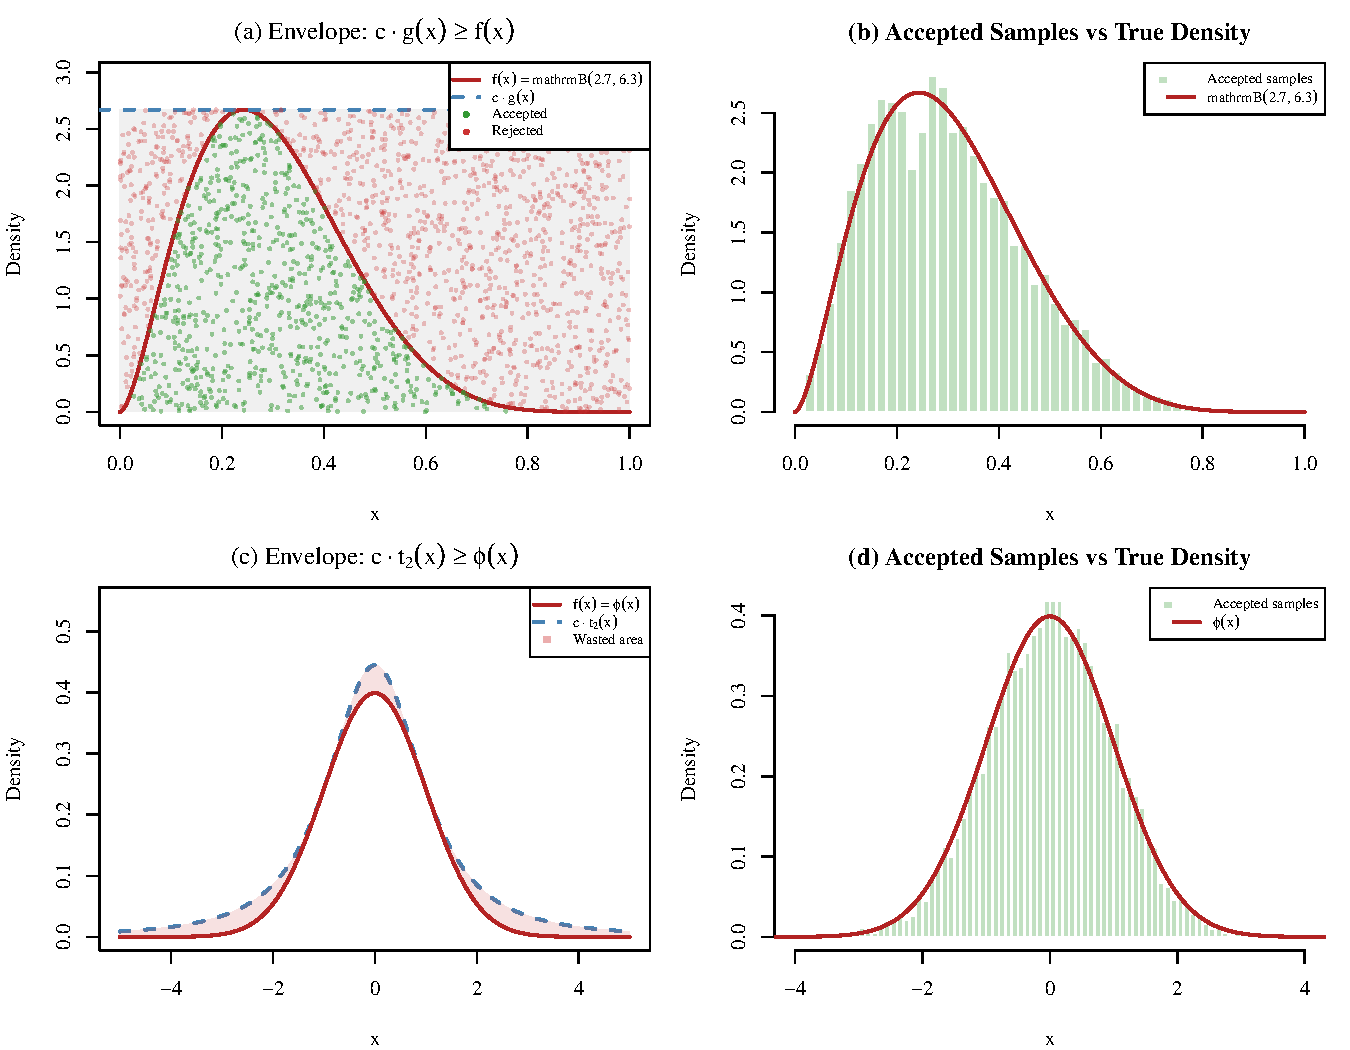
\includegraphics[width=\textwidth]{plots/fig_envelopes.pdf}
  \caption{%
    \textbf{(a)}~Dart-board visualization for the $\mathrm{Beta}(2.7,6.3)$ target with a $\mathrm{Uniform}(0,1)$ proposal.
    Green points fall under $f(x)$ and are accepted; red points are rejected.
    \textbf{(b)}~Histogram of accepted samples overlaid with the true Beta density.
    \textbf{(c)}~Envelope $c\cdot t_2(x)$ over the standard normal target $\phi(x)$; the shaded region is wasted probability.
    \textbf{(d)}~Histogram of accepted samples vs.\ $\phi(x)$.
  }
  \label{fig:envelopes}
\end{figure}

% ----------------------------------------------------------------
\subsection{Figure~\ref{fig:efficiency}: Efficiency vs.\ Envelope Constant}

The acceptance rate is exactly $1/c$.  Figure~\ref{fig:efficiency} plots this relationship for a range of $c$ values above the optimal $c^*$, illustrating why minimizing $c$ matters.  Choosing $c$ even $2\times$ too large cuts efficiency in half.

\begin{lstlisting}
c_vals <- seq(c_beta, c_beta * 3, length.out = 30)
eff <- 1 / c_vals
plot(c_vals, eff * 100, type = "b", ...)
\end{lstlisting}

\begin{figure}[H]
  \centering
  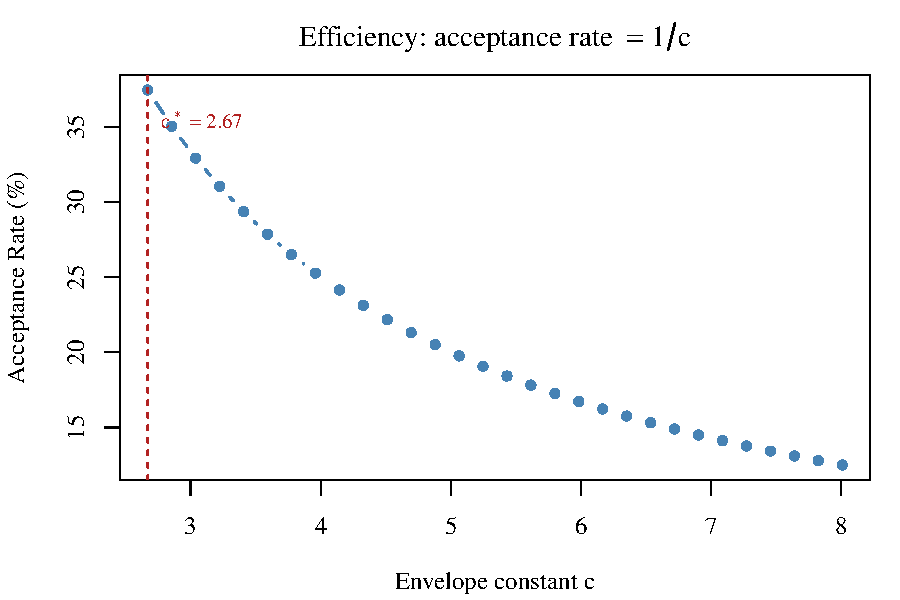
\includegraphics[width=0.75\textwidth]{plots/fig_efficiency.pdf}
  \caption{Acceptance rate $1/c$ as a function of the envelope constant~$c$.  The dashed vertical line marks the optimal $c^* \approx 2.67$ for the $\mathrm{Beta}(2.7,6.3)$/Uniform example.  Larger~$c$ wastes more proposals.}
  \label{fig:efficiency}
\end{figure}

% ----------------------------------------------------------------
\subsection{Figure~\ref{fig:steps}: Step-by-Step Visualization}

The final figure isolates six individual iterations of Algorithm~\ref{alg:reject}.  For each step:
\begin{enumerate}
  \item A proposal $x$ is drawn from $g$ (the $x$-coordinate).
  \item A uniform $u$ is drawn; the point $(x, u \cdot c)$ is plotted.
  \item If the point falls \emph{under} $f(x)$, the panel is labeled ``Accept''; otherwise ``Reject.''
  \item An arrow from the $x$-axis to the point illustrates the ``dart throw.''
\end{enumerate}
Previous points accumulate across panels, building intuition for how the sample grows.

\begin{lstlisting}
for (k in 1:steps) {
  # ... draw envelope and target ...
  pt_col <- ifelse(acc_seq[k], "green4", "red3")
  points(x_seq[k], u_seq[k] * c_beta,
         pch = 8, cex = 2, col = pt_col, lwd = 2)
  arrows(x_seq[k], 0, x_seq[k], u_seq[k] * c_beta,
         length = 0.08, col = pt_col, lty = 3)
}
\end{lstlisting}

\begin{figure}[H]
  \centering
  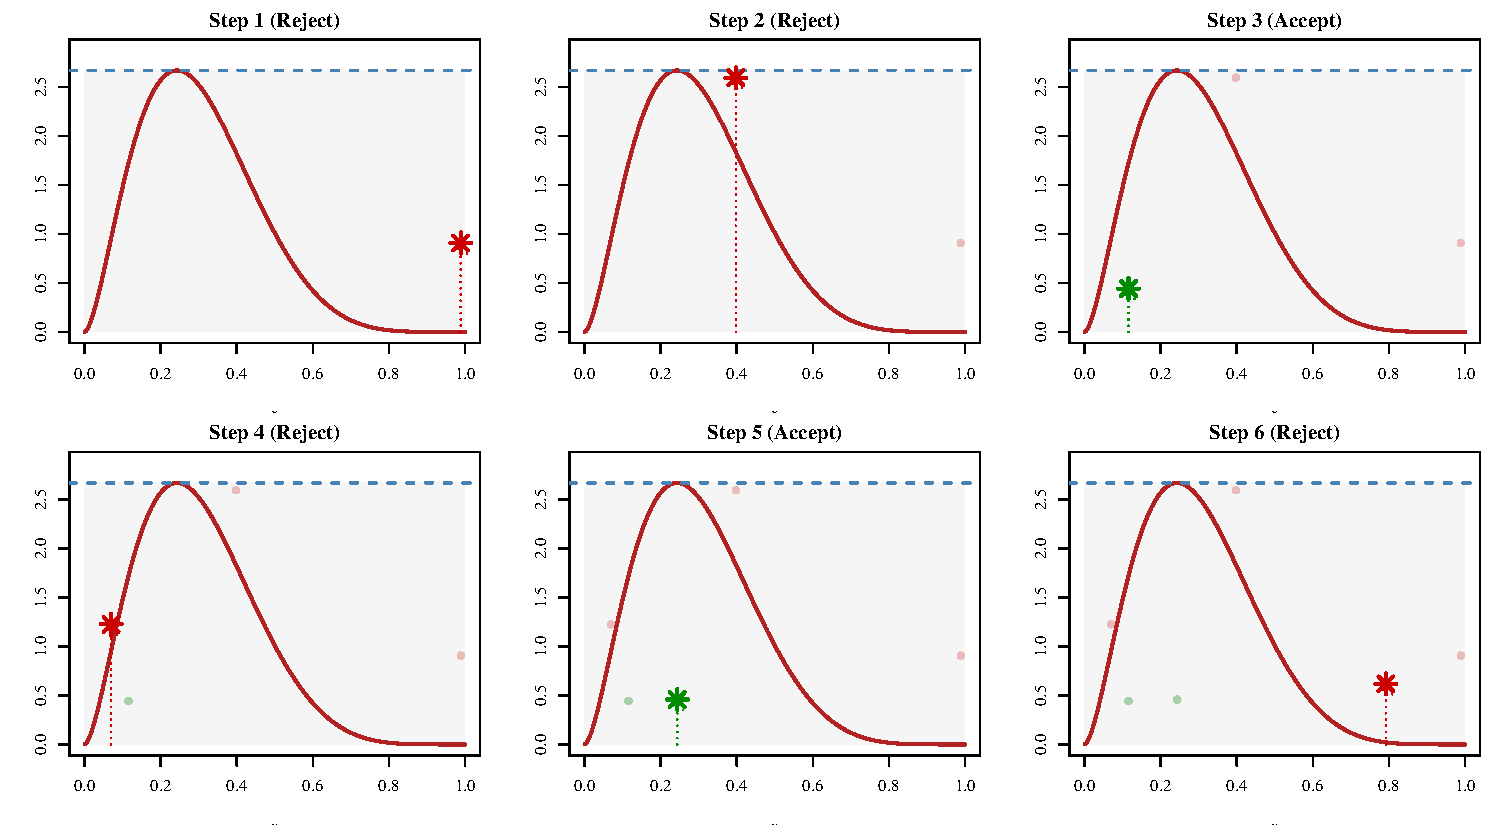
\includegraphics[width=\textwidth]{plots/fig_steps.pdf}
  \caption{Six sequential iterations of rejection sampling for $\mathrm{Beta}(2.7,6.3)$.  Each panel adds one proposal: a star marks the current draw, with an arrow from the $x$-axis showing its height $u \cdot c$.  Green~=~accepted (under the curve), red~=~rejected (above).  Previous points accumulate across panels.}
  \label{fig:steps}
\end{figure}

% ----------------------------------------------------------------
\section{The 2D Picture: Contour Visualization}

To build geometric intuition, we apply rejection sampling to a two-dimensional target $p(\mathbf{x}) = N(\mathbf{0}, I_2)$ using a uniform proposal on $[-3,3]^2$.  In 2D the ``dart-board'' is a square, and accepted points cluster inside the circular contours of the bivariate normal.

\paragraph{Figure~\ref{fig:contour2d}(a): 2D accept/reject.}
Green points falling inside the high-density contours are accepted; red points in the corners of the bounding box are rejected.  The wasted area in the corners is already substantial in two dimensions.

\paragraph{Figure~\ref{fig:contour2d}(b): Curse of dimensionality.}
Panel~(b) plots the theoretical acceptance rate $1/c = (\sqrt{2\pi}/6)^d$ as a function of dimension~$d$ for the same $N(\mathbf{0},I_d)$/Uniform setup.  At $d=1$ the acceptance rate is $\approx 41.7\%$; by $d = 10$ it is below $0.02\%$.  This exponential decay is why rejection sampling is impractical beyond a handful of dimensions.

\begin{lstlisting}
# Theoretical acceptance rate for N(0,I_d) with Uniform[-3,3]^d
acc_rates[di] <- (sqrt(2 * pi) / 6)^d
\end{lstlisting}

\begin{figure}[H]
  \centering
  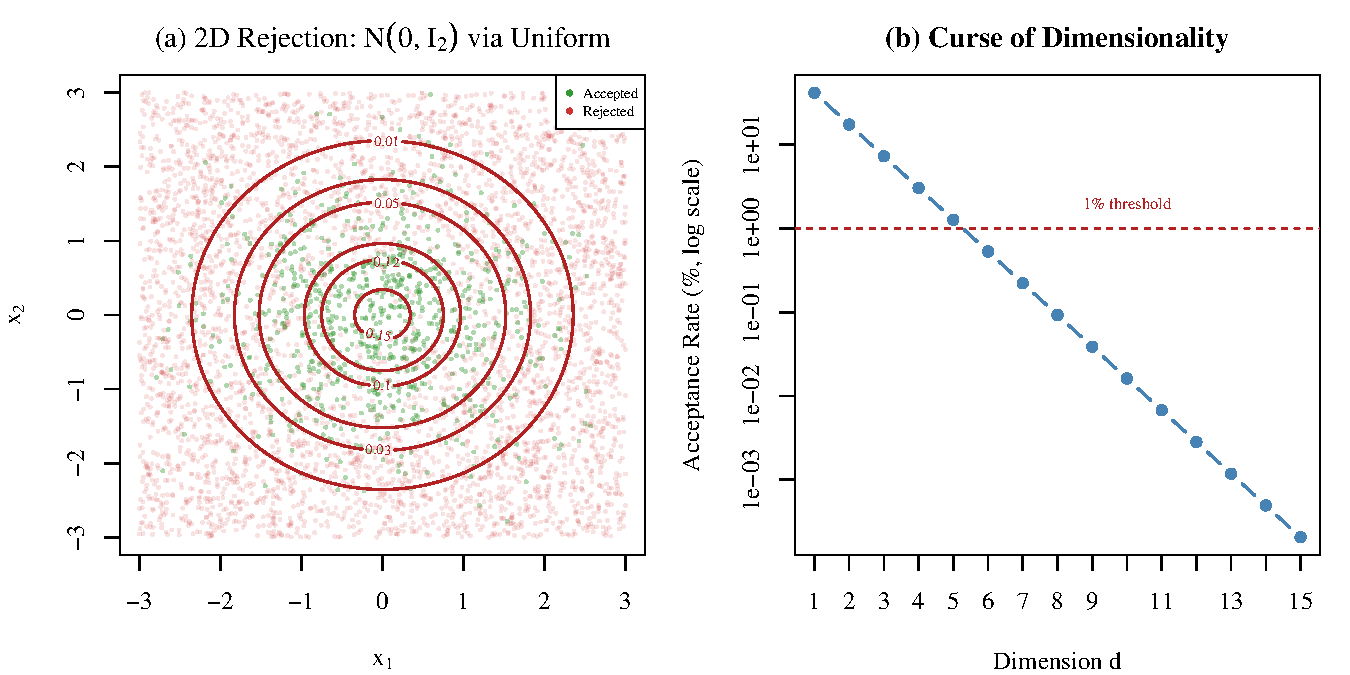
\includegraphics[width=\textwidth]{plots/fig_contour_2d.pdf}
  \caption{%
    \textbf{(a)}~Rejection sampling on a bivariate $N(\mathbf{0},I_2)$ target with a uniform proposal on $[-3,3]^2$.  Accepted samples (green) concentrate inside the density contours; rejected samples (red) fill the wasted corners.
    \textbf{(b)}~Acceptance rate decays exponentially with dimension: at $d=10$ it is below $0.02\%$.
  }
  \label{fig:contour2d}
\end{figure}

% ----------------------------------------------------------------
\section{Where Rejection Sampling Fails}

\subsection{Failure Mode: No Finite Envelope Exists}

Rejection sampling requires a finite constant $c$ such that $c\cdot g(x) \ge f(x)$ for \emph{all}~$x$.  This condition is violated when the target $f$ has \textbf{heavier tails} than the proposal~$g$.

\paragraph{Example.}
Let the target be $f(x) = \mathrm{Cauchy}(0,1)$ and the proposal be $g(x) = N(0,1)$.  As $|x| \to \infty$,
\[
  \frac{f(x)}{g(x)} = \frac{(1/\pi)(1+x^2)^{-1}}{(2\pi)^{-1/2}\,e^{-x^2/2}}
  \;\sim\; \frac{\sqrt{2\pi}}{\pi}\,\frac{e^{x^2/2}}{1+x^2}
  \;\to\; \infty.
\]
No finite $c$ can contain this ratio.  Figure~\ref{fig:rs-failure}(a) shows the Cauchy density poking above any scaled normal envelope in the tails, and Figure~\ref{fig:rs-failure}(b) confirms the ratio $f(x)/g(x)$ diverges.

\paragraph{Fix.}
Reverse the roles: use $g = \mathrm{Cauchy}$ to sample from $f = N(0,1)$.  More generally, the proposal must always have \textbf{at least as heavy tails} as the target.  If no such $g$ is available (e.g., the target's tail behavior is unknown), rejection sampling cannot be applied and one must turn to MCMC or importance sampling.

\begin{figure}[H]
  \centering
  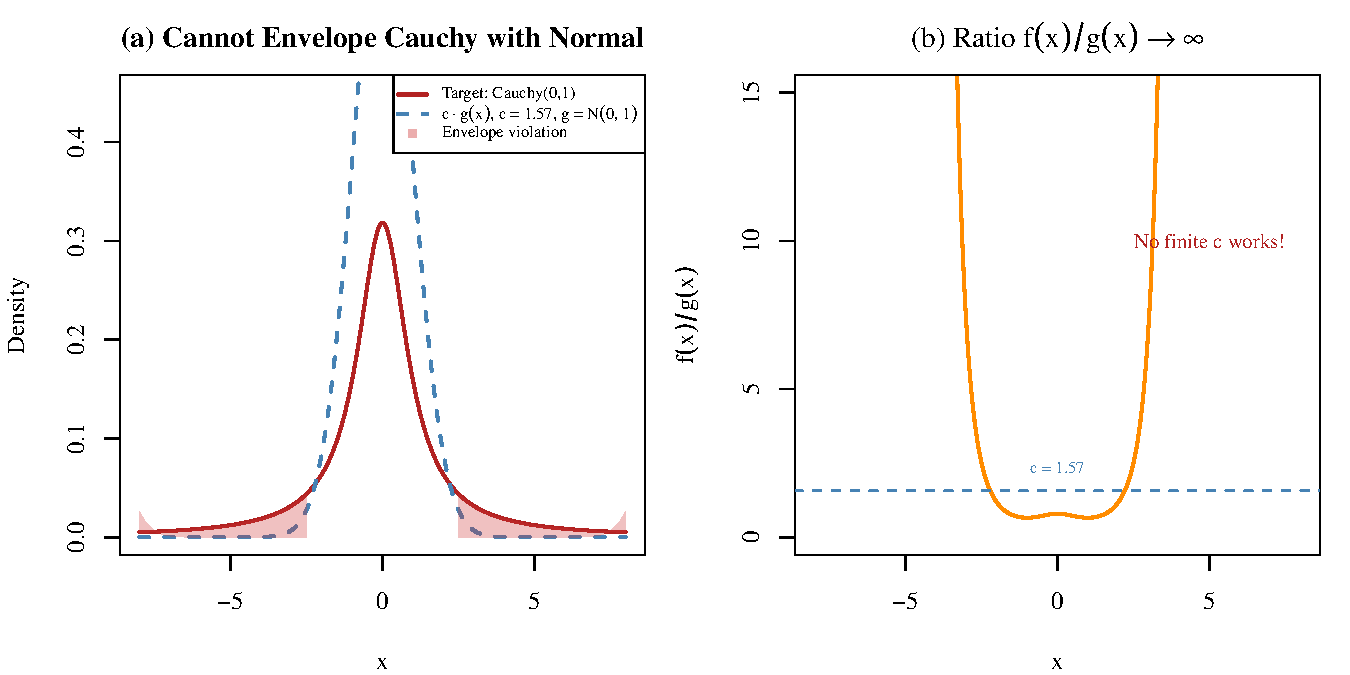
\includegraphics[width=\textwidth]{plots/fig_rs_failure.pdf}
  \caption{%
    \textbf{(a)}~Attempting to envelope the Cauchy target (red) with a scaled normal (blue dashed).  The shaded regions mark where the envelope is violated---no finite $c$ fixes this.
    \textbf{(b)}~The ratio $f(x)/g(x) = \mathrm{Cauchy}(x)/\phi(x)$ diverges in the tails, confirming the impossibility.
  }
  \label{fig:rs-failure}
\end{figure}

% ----------------------------------------------------------------
\section{Key Takeaways}

\begin{itemize}
  \item Rejection sampling produces \textbf{exact, independent} draws from $f$---no burn-in or autocorrelation.
  \item Efficiency is governed entirely by the constant~$c$: acceptance rate $= 1/c$.
  \item In \textbf{low dimensions}, a good proposal $g$ that closely matches $f$ makes rejection sampling practical.
  \item In \textbf{high dimensions}, the ratio of the volume under $f$ to the volume under $c\cdot g$ shrinks exponentially, making acceptance rates vanishingly small.  This motivates MCMC methods (Metropolis--Hastings, Gibbs) that sacrifice independence for guaranteed samples.
  \item The Uniform proposal in Example~1 ($1/c \approx 37.5\%$) is far less efficient than the $t_2$ proposal in Example~2 ($1/c \approx 79.5\%$), illustrating the importance of matching the proposal shape to the target.
  \item Rejection sampling \textbf{cannot} be used when the proposal has lighter tails than the target (e.g., normal proposal for a Cauchy target)---no finite $c$ exists.
\end{itemize}

\end{document}
